\section{Manufacturer's Product Literature}
\label{app:manufacturer}

The pressure relief device we use for SLArPAAS I is a MDC precision 
burst disc with the cracking pressure at 9--11.5~psig.
Manufacturer's document can be found in Fig.~\ref{fig:mdc_burst_disc} and at
\url{https://www.mdcprecision.com/420033-asme-pressure-burst-disc-9-11-5-psig-dn40cf-275cf-316lss}.\\

The manufacturer's documents for the back pressure regulator and the check valve
are shown in Figs.~\ref{fig:swagelok_bpr_1}, \ref{fig:swagelok_bpr_2},
and \ref{fig:generant_cv}.\\

% --------------------------------------------------------
\begin{figure}[h]
    \centering
    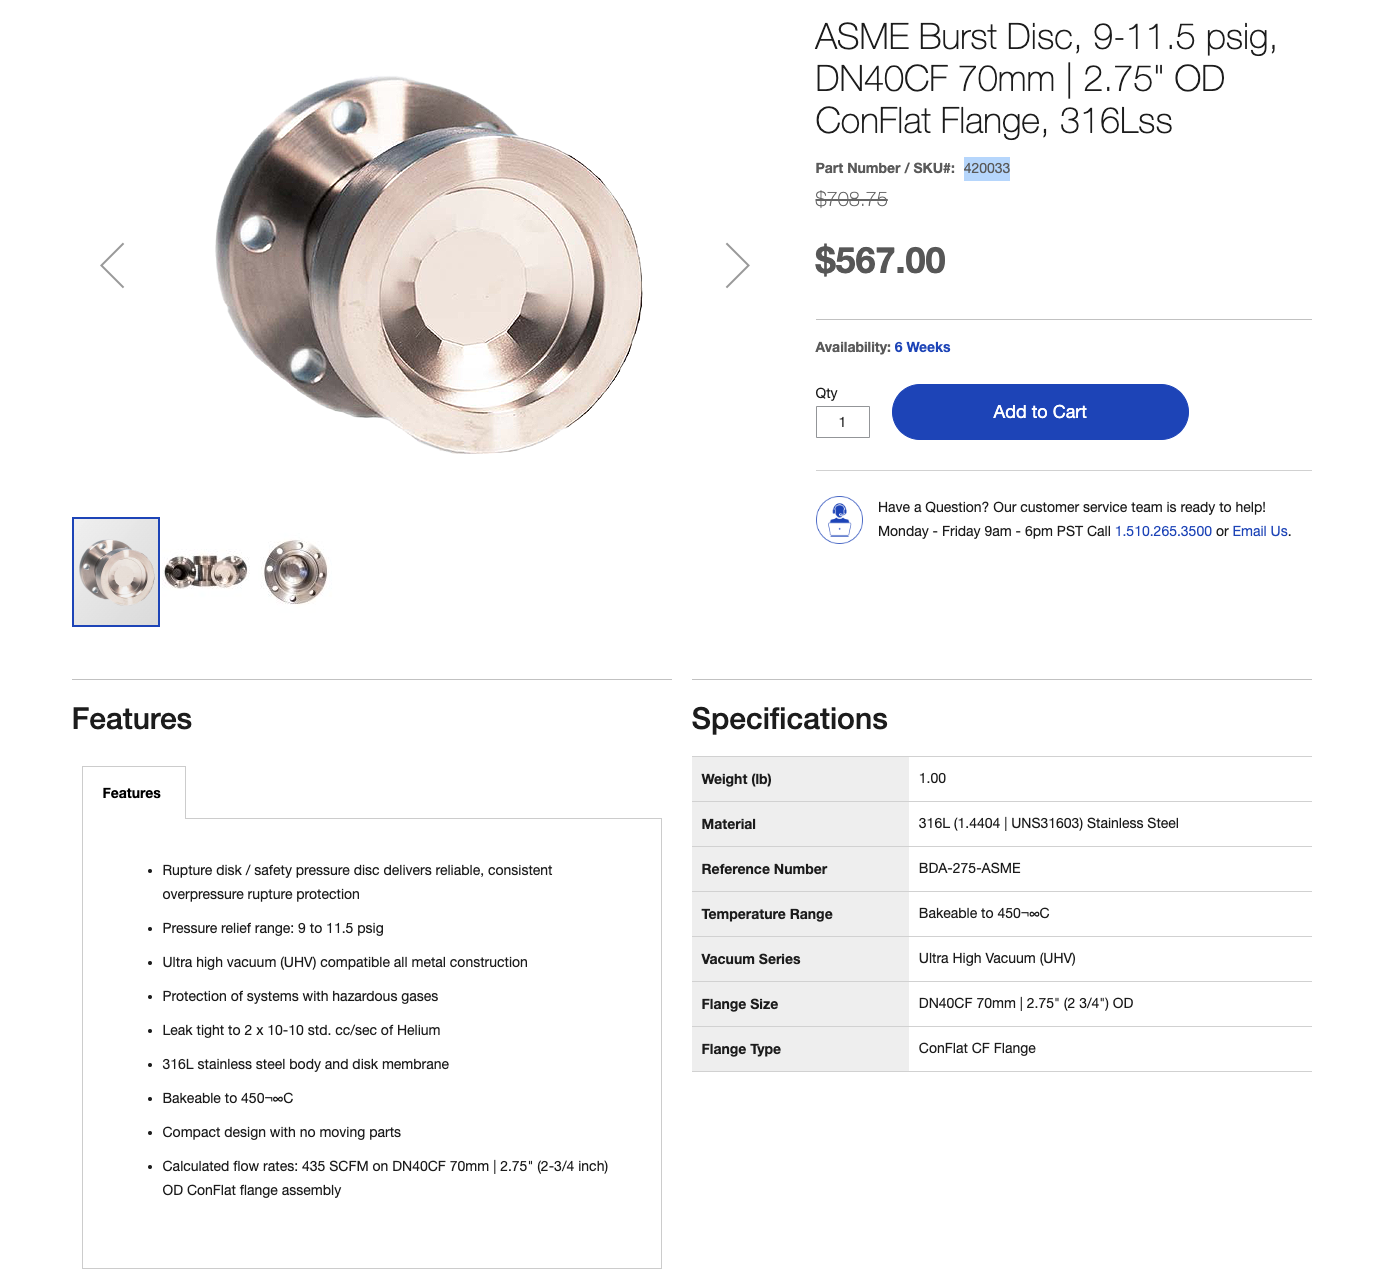
\includegraphics[width=0.75\textheight]{fig/MDC_BurstDisc.png}
    \caption{Manufacturer's information of the burst disc.}
    \label{fig:mdc_burst_disc}
\end{figure}
% --------------------------------------------------------

% --------------------------------------------------------
\begin{figure}[h]
    \centering
    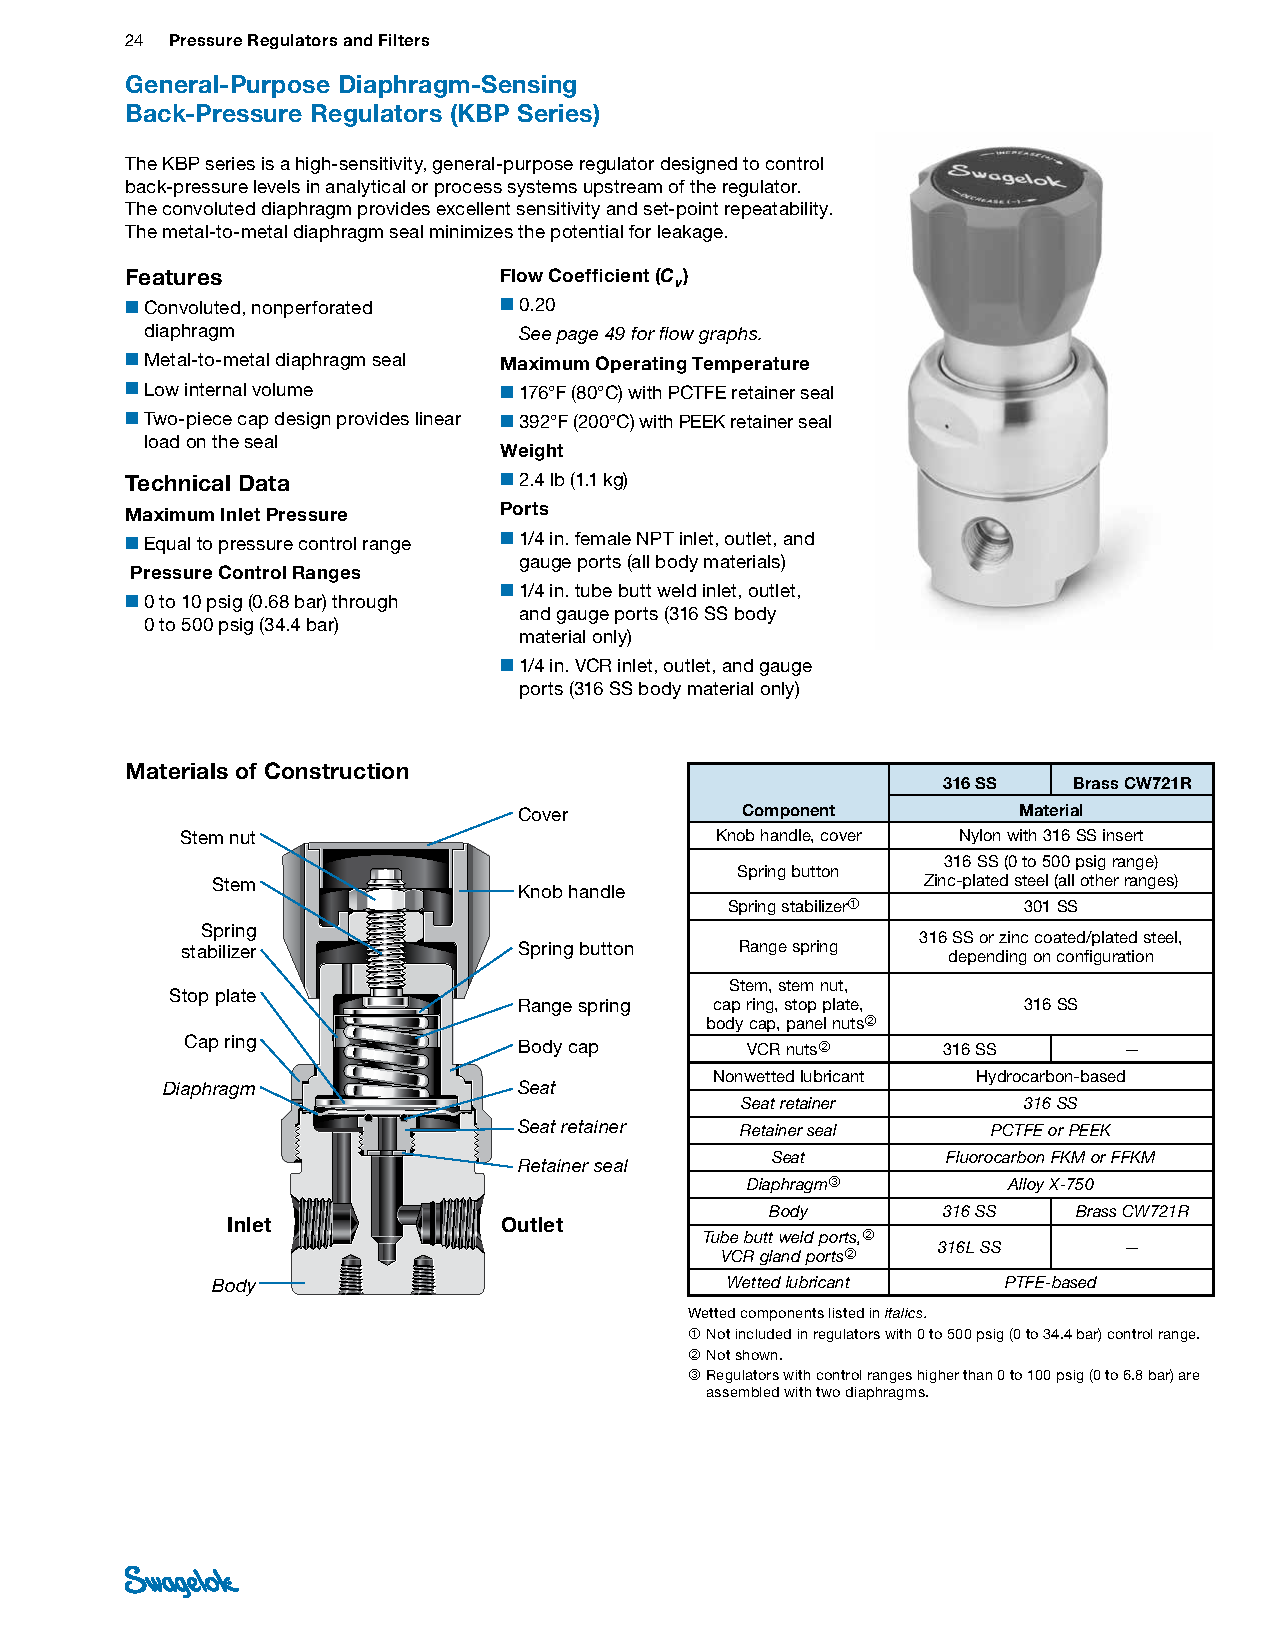
\includegraphics[width=\textwidth]{fig/BPR-1.pdf}
    \caption{First part of the manufacturer's information of the back pressure regulator.}
    \label{fig:swagelok_bpr_1}
\end{figure}
% --------------------------------------------------------

% --------------------------------------------------------
\begin{figure}[h]
    \centering
    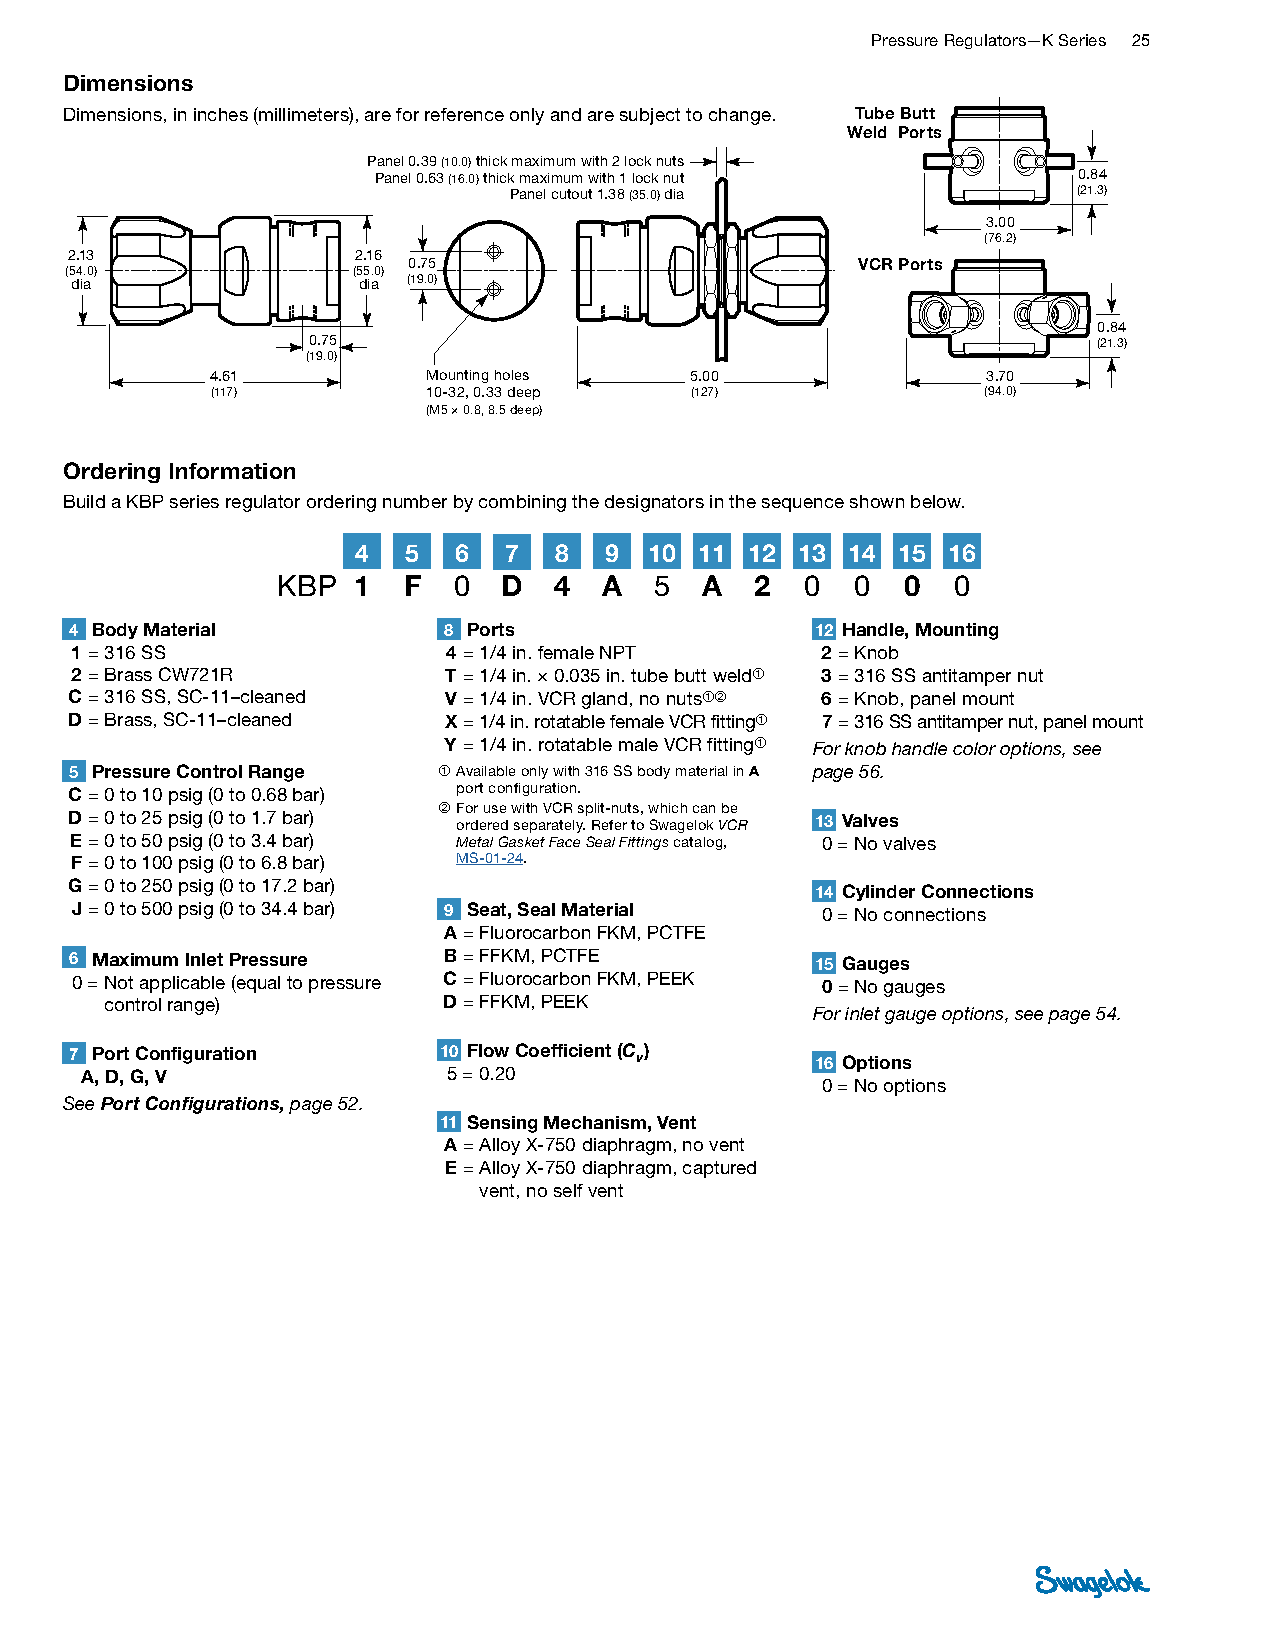
\includegraphics[width=\textwidth]{fig/BPR-2.pdf}
    \caption{Second part of the manufacturer's information of the back pressure regulator.}
    \label{fig:swagelok_bpr_2}
\end{figure}
% --------------------------------------------------------

% --------------------------------------------------------
\begin{figure}[h]
    \centering
    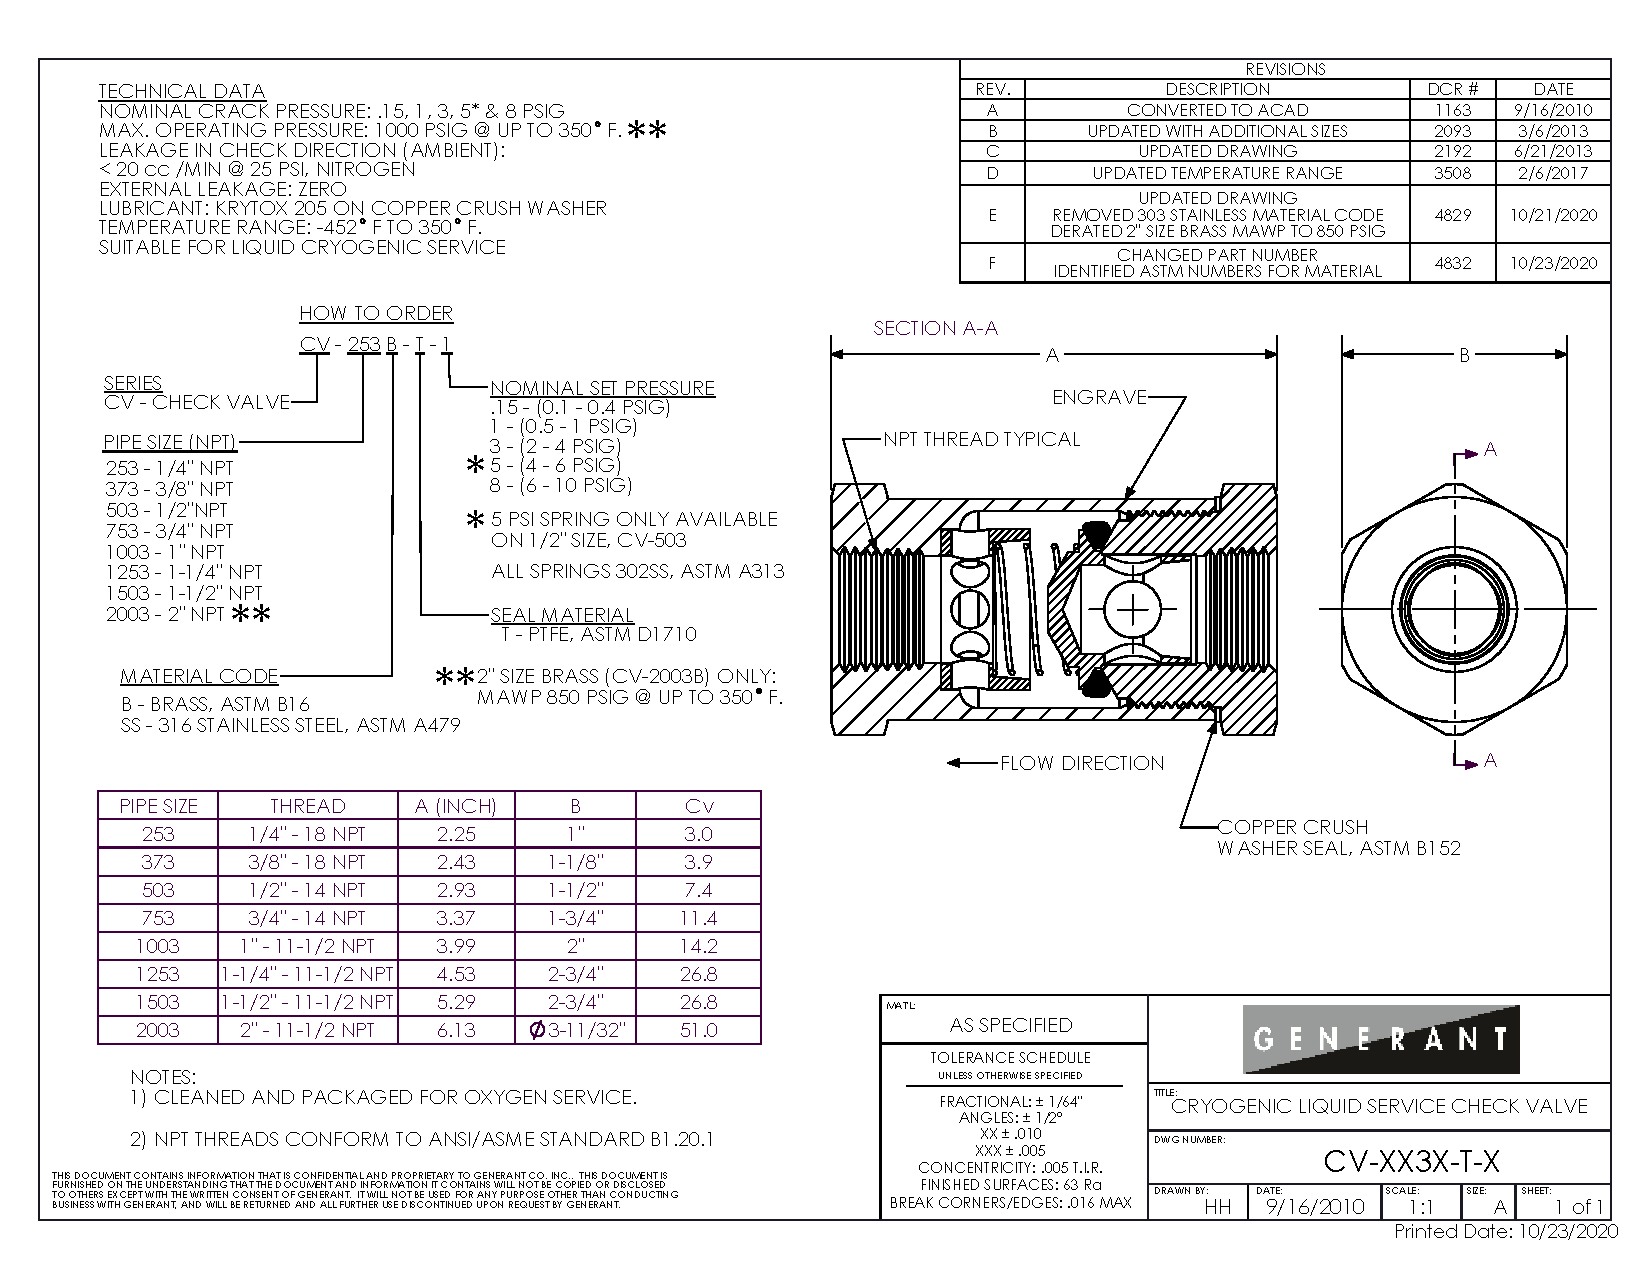
\includegraphics[width=\textwidth]{fig/CV-XX3X-T-X.pdf}
    \caption{Manufacturer's information of the check valve.}
    \label{fig:generant_cv}
\end{figure}
% --------------------------------------------------------
